\documentclass[main.tex]{subfiles}

\begin{document}
	
	\begingroup
	
	\renewcommand{\cleardoublepage}{}
	
	\renewcommand{\clearpage}{}
	
	\chapter{Storing Groceries Task Overview}
	\label{grocery-sequence}
	
	\chapterauthor{Torge Olliges, Tom-Eric Lehmkuhl, \\Evan Kapitzke, Jeremias Thun, Jan Neumann}

	\section{Goal}
	The goal of the Storing Groceries task is, like the name indicates, to store several groceries at their designated position. For the RoboCup this task has been simplified. The objects are all on a table and need to be sorted into a predefined shelf. The sorting has to be done by categories which need to be comprehensible by a human. This can be based on color, form, or other categories. To fulfill this task the HSR has to identify the objects on the table and existing objects on the shelf. Furthermore it needs to grasp and place one object after the other. It also needs to navigate between the shelf and the table. For additional points the HSR has to open doors. Overall the HSR has only 5 minutes to complete the task. 

	\section{Tasks}
	The figures \ref{grocery_seq_01} and \ref{grocery_seq_02} show the procedure of Storing Groceries. The following subsections explain the execution and procedure in detail and give insights into the decisions made resulting in the exact plan depicted below. Additionally a more in-depth explanation of some of the challenges will be given. To make the written version more reader-friendly, there is not every single call and answer mentioned, only the ones necessary to understand the sequence of this task.\\
	To keep it clear which task is done by which group, the tasks are labled with colors:\\
	~\\
	
	\begin{planning}
	Planning group
	\end{planning}
	\begin{knowledge}
	Knowledge group
	\end{knowledge}
	\begin{navigation}
	Navigation group
	\end{navigation}
	\begin{manipulation}
	Manipulation group
	\end{manipulation}
	\begin{perception}
	Perception group
	\end{perception}
	\begin{nlp}
	NLP group
	\end{nlp}
	
		\begin{figure}[H]
			\centering
			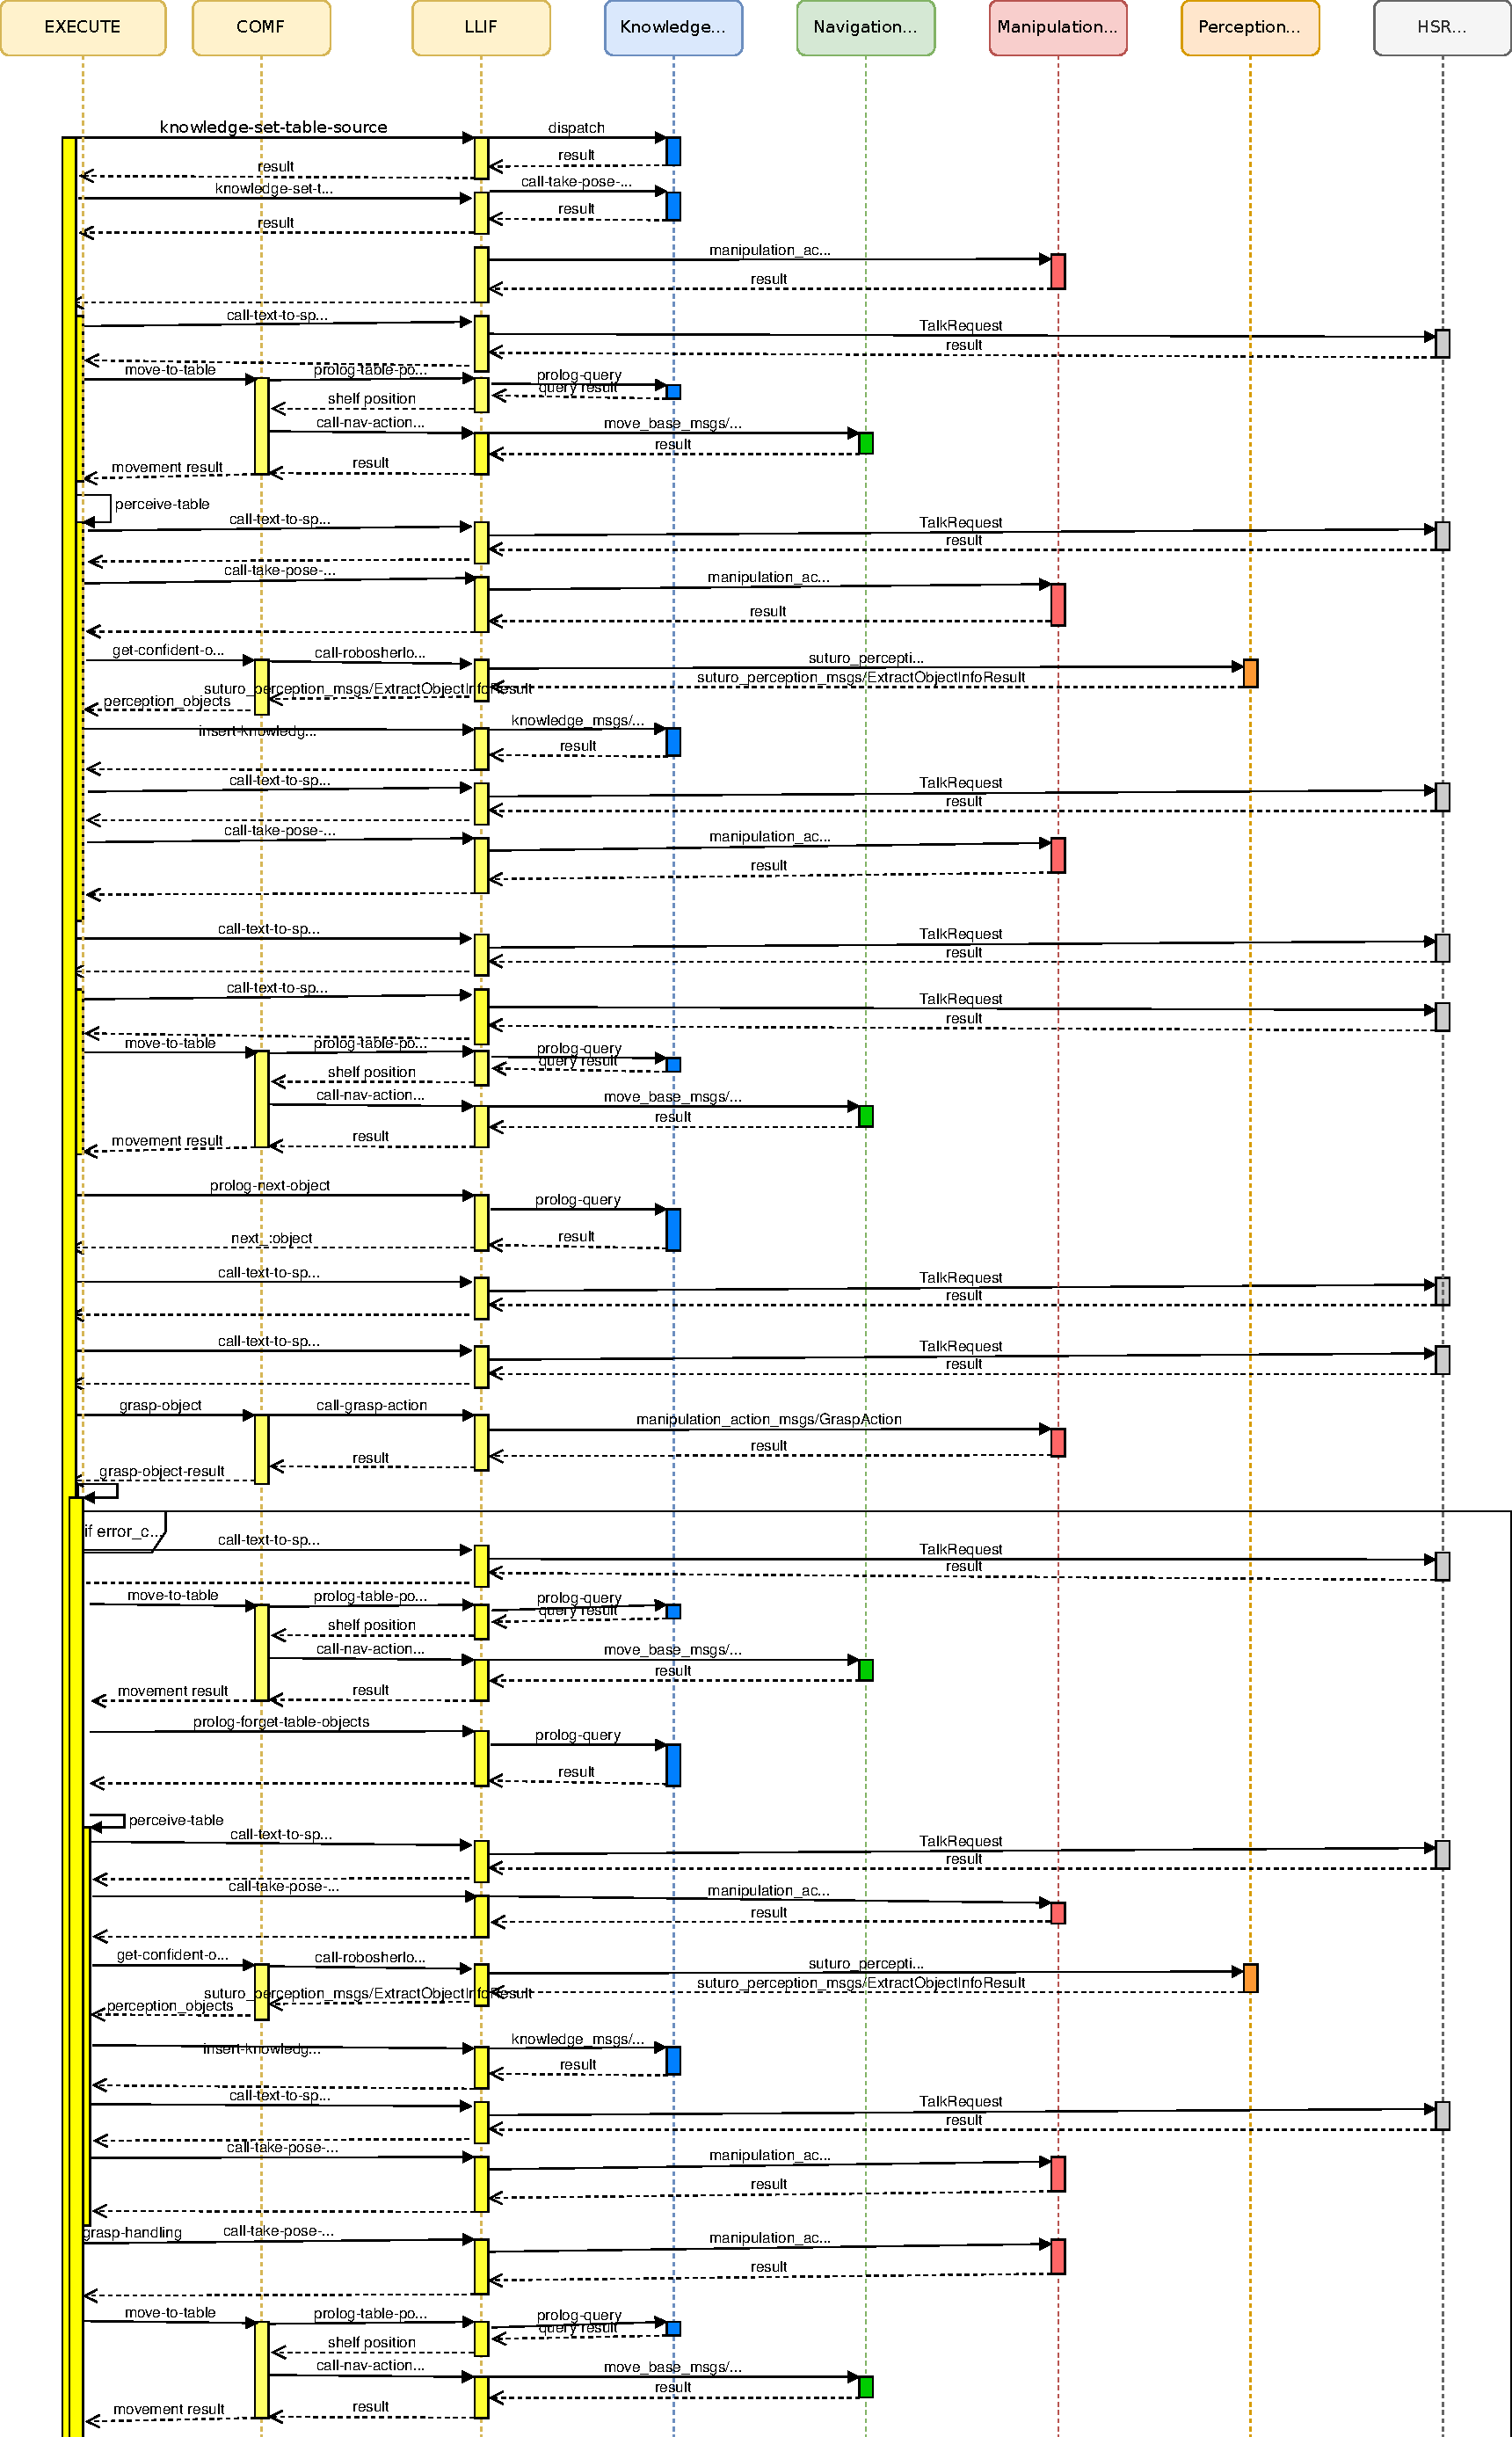
\includegraphics[width=0.9\textwidth]{pictures/diagramms/grocery_01_seq}
			\caption{Sequence diagram of the complete run of the grocery storing task \textit{(explanations below)}}
			\label{grocery_seq_01}
		\end{figure}
		\begin{figure}[H]
			\centering
			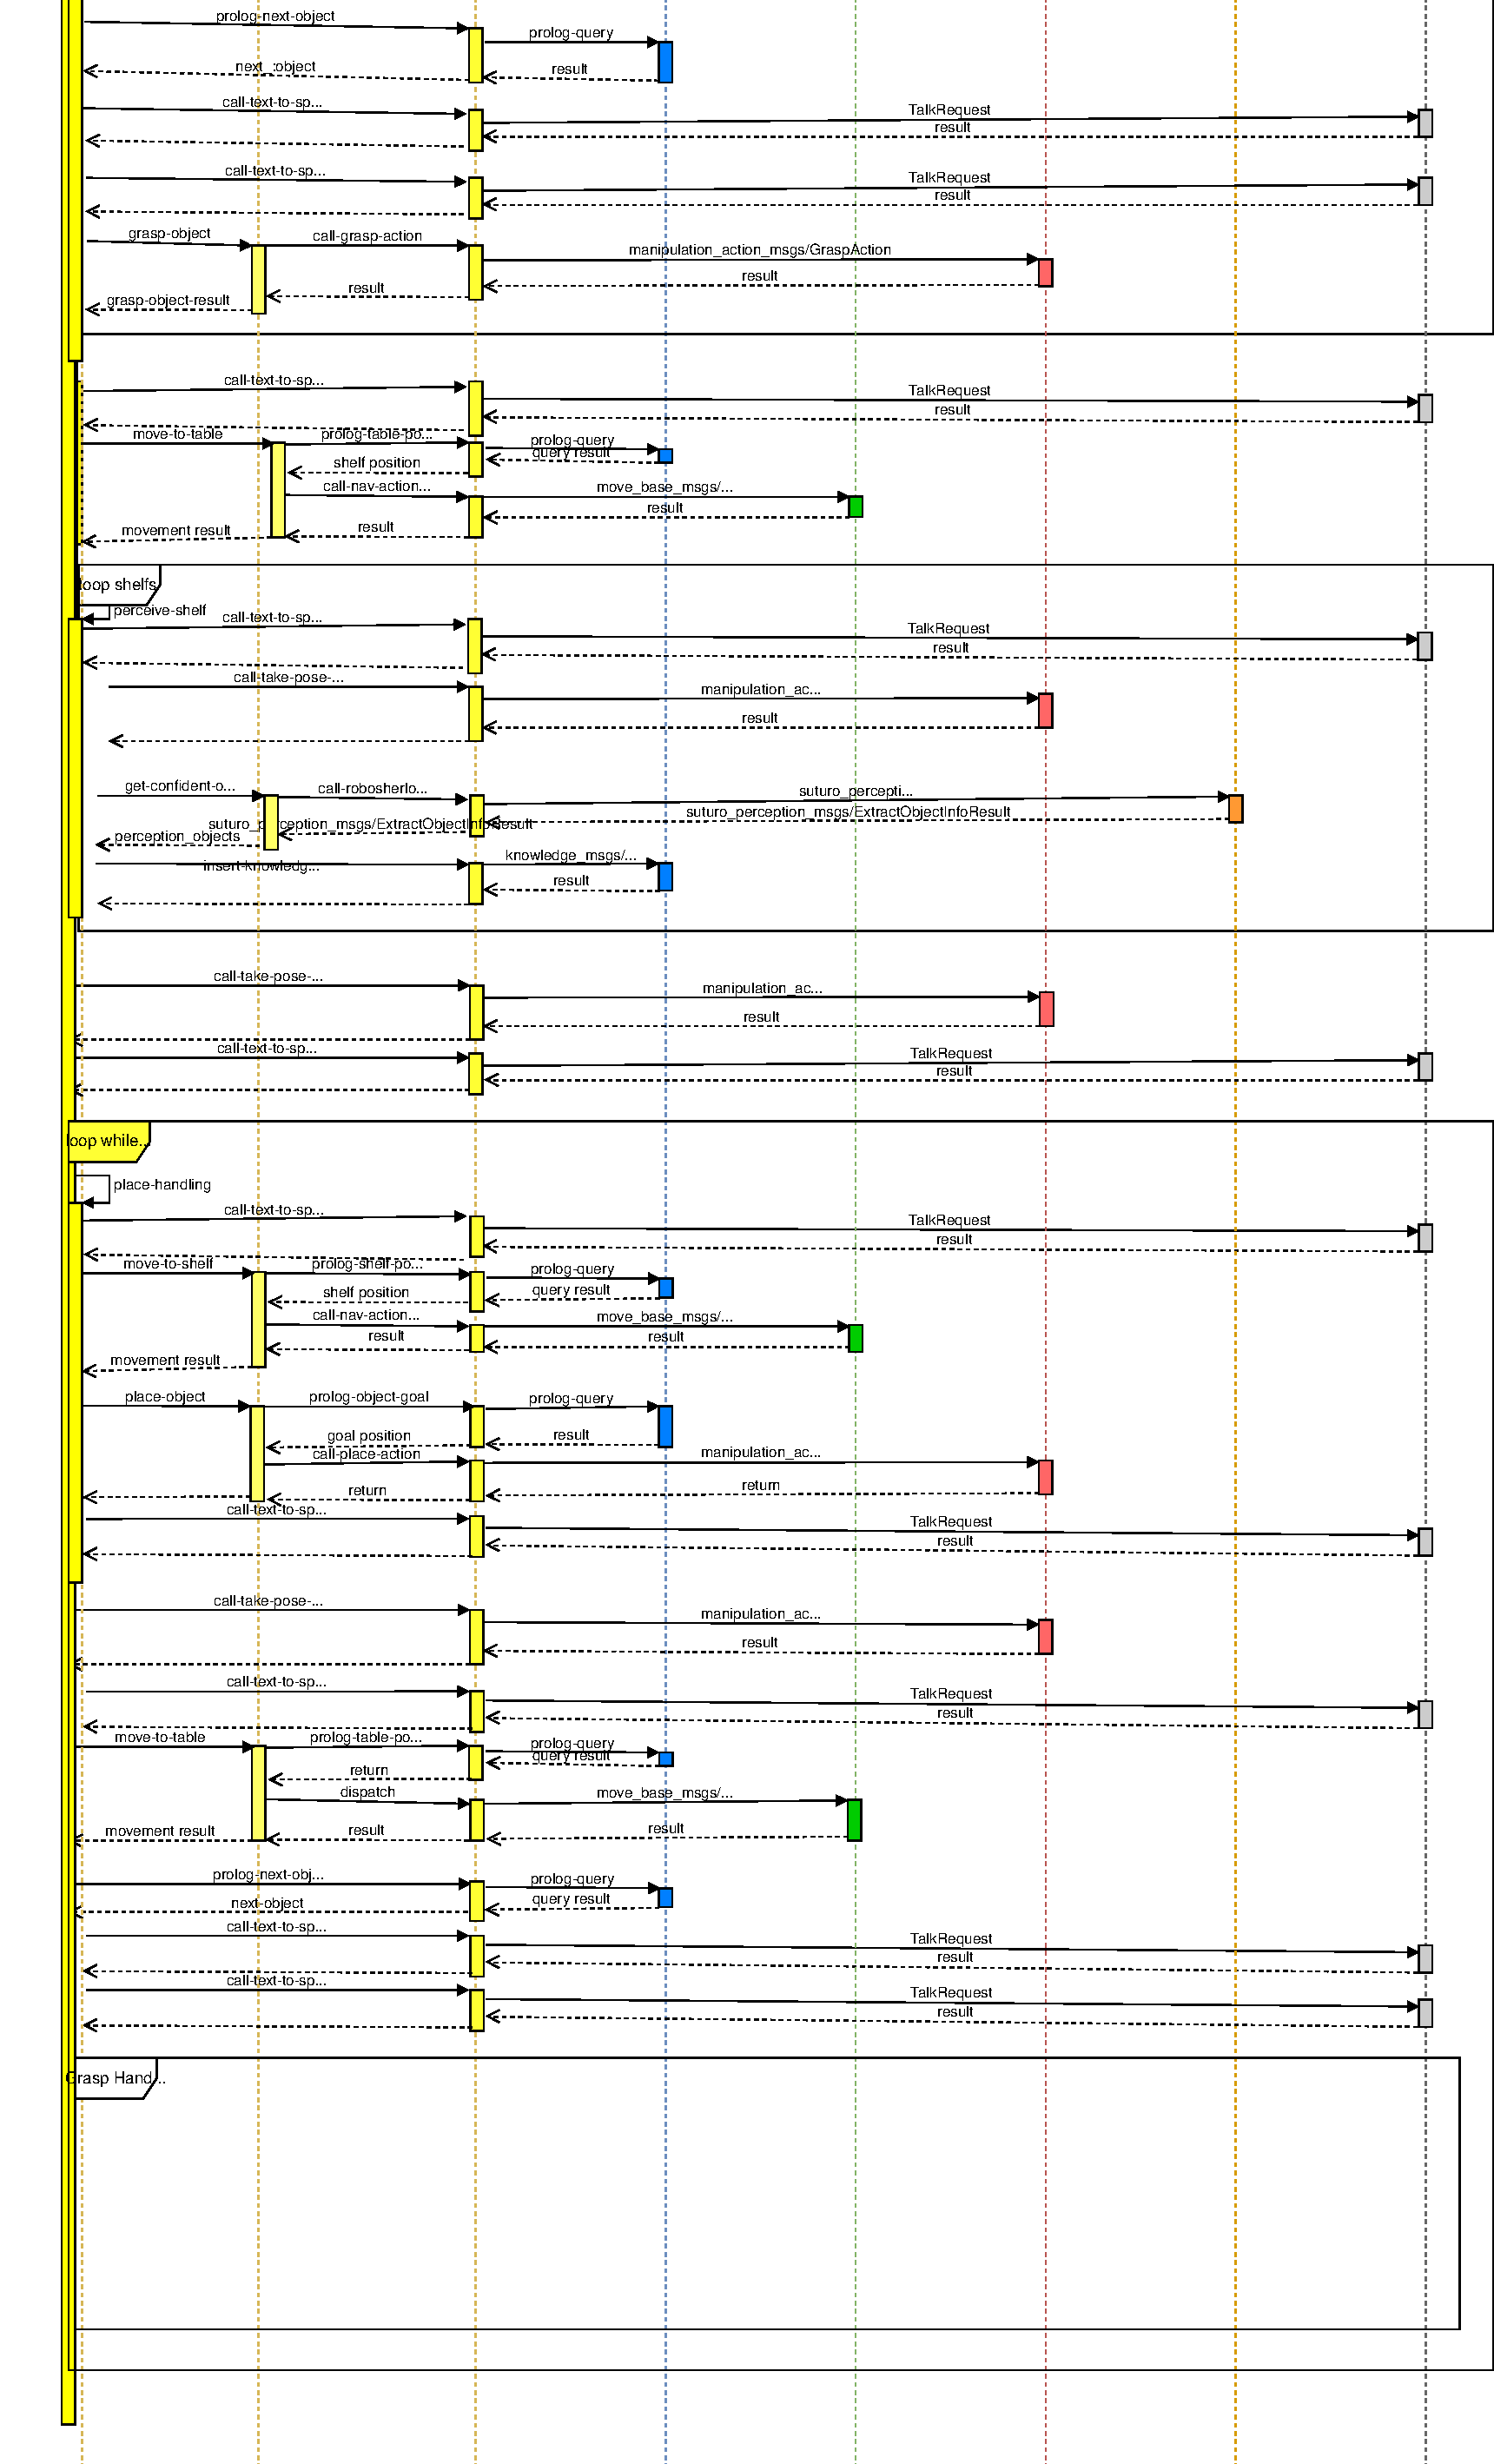
\includegraphics[width=0.9\textwidth]{pictures/diagramms/grocery_02_seq}
			\caption{Sequence diagram of the complete run of the grocery storing task \textit{(explanations below)}}
			\label{grocery_seq_02}
		\end{figure}
		\textit{The sequence diagram in figure \ref{grocery_seq_01} and \ref{grocery_seq_02} does not depict when the action servers are running it rather displays the time they are actively used.}
	
	\subsection{Setup}
	

	% Knowledge: set-tables-source 
	\begin{knowledge}
	According to the task only one table serves as the \texttt{source} for objects. In Knowledge it is allowed to set multiple \texttt{sources} for objects to allow greater compatibility and easier adaption to other tasks. For the current task at hand only the corresponding table is set as \texttt{source}. The same principle applies to the shelf which is set as \texttt{target} surface. Every surface e.g. tables, shelf's or the floor can be set as \texttt{source} or \texttt{target}.
	\end{knowledge}
	
		% Manipulation: take pose action
	\begin{manipulation}
	The robot is set to the default pose to make sure it is in a neutral state. This is important to avoid moving the robot for example with an extended arm. Manipulation allows the use of predefined poses as well as setting a pose by defining the joint states these informations are sent via th \nameref{msg_take_pose} action. These joint states are then forwarded to \textit{Giskard}.\end{manipulation}
	
	\subsection{Scan table sequence}
	
	% NLP: Talk Request
	\begin{nlp}
	To inform the developer as well as the people following the robot or evaluating its behavior about what the robot is about to do, the robot will talk about its actions. These talk requests are also used for safety measures so the robot can warn when it is going to move so bystanders can step aside. \end{nlp}
	
	% Knowledge: get table-poses
	\begin{knowledge}
	To start the task, Knowledge finds all the tables available, sorts them by their distance to the robot and then returns the list of their position to Planning, so that Planning can determine where the robot has to go first.\end{knowledge}
	
	% Navigation: moveBaseAction
	\begin{navigation}
	Planning determines a goal for the \nameref{msg_move_base} action. For this specific goal the robot is turned $90^\circ$ and moved to the nearest table, allowing it to look over its shoulder having a clear view of the table without the arm in its way. The default navigation client of the HSR executes the action. \end{navigation}
	
	% NLP
	\begin{nlp}
	The robot then says that it is starting to perceive the table.\end{nlp}
	
	% Manipuilation: TakePoseAction
	\begin{manipulation}
	Manipulation gets the task to put the robot into a pose to perceive an object depending on the height of the plane the object is on.
    That is necessary for Perception to get a good angle and distance to the object and to avoid having the robots arm block the camera's view.
    \end{manipulation}
	
	% Perception: Percieve and return data
	\begin{perception}
	The HSR takes a picture of the scene it is currently looking at and processes it with RoboSherlock. Based on the requested region the input images are filtered. As a result, Perception provides various data about the objects standing on the table, including their category (Pringles / Coke can / Apple / ...), their position, and their dimensions. These results are then published by the \textit{perception\_actionserver} so planning can find them.\end{perception}
	
	% Planning confident check
	\begin{planning}
	Planning checks the confident values of detected objects and sorts out objects with too much uncertainty. The data is then transferred to Knowledge.
	\end{planning}
	
	% Knowledge: Store Data
	\begin{knowledge}
	Knowledge verifies the data of the objects, that were perceived and are supposed to be stored. If the class of an object is unknown to Knowledge or if it could not have been perceived with a high enough confidence, it is set to the class \texttt{Other}, if the dimensions are too small to be an object, it is rejected and so on. If the data for the given object is valid, the object gets added to the Knowledge base. Should the objects stand close to one another, they get organized in a group. Groups are used to sort objects and can be used to determine if an object is hard to grasp.
	\end{knowledge}
	% NLP: Talk Request
	
	% Manipulation: Take pose
	\begin{manipulation}
	To grasp an object the HSR needs to look straight at the object with its base. Therefore the HSR needs to be in its default pose allowing safe movement.
	\end{manipulation}
	% 2x NLP: Talk
	
	% Knowledge: prolog_ table_pose
	\begin{knowledge}
	For Planning to give the orders to move the robot to the table with the object to grasp on it, Knowledge once again provides the position data of the nearest table.
	\end{knowledge}
	
	% Navigation: MoveBaseAction
	\begin{navigation}
	Turn the HSR by $90^\circ$ so it looks straight at the table and can grasp an object.
	\end{navigation}
	
	\subsection{Grasp sequence}
	
	\label{grasp-object}
	% Knowledge: next_object
	\begin{knowledge}
	Knowledge now determines which object should be grasped next, to place it in one of the shelves. This decision is purely based on the distance of the objects to the robot so that the nearest object standing on the table will be taken first. This is one of the parts with a lot of ideas on how it can be improved in the future, as will be discussed in section \ref{sec:nextObj}.
	\end{knowledge}
	
	% 2x NLP: Talk Request
	\begin{nlp}
	The HSR says which object will be grasped. The object name is the object identifier without the unique string prefix for the knowledge base.
	\end{nlp}
	
	% Manipulation: GraspAction
	\begin{manipulation}
	Manipulation gets the task to grasp the given object. Different modes of grasping are possible but at the moment only frontal grasping is used actively. At first the orientation of the gripper is calculated based on the HSR's rotation. Additionally the collision for the object to grasp gets deactivated. This is important since otherwise \textit{Giskard} would stop the gripper in front of the object. During the project it became apparent that \textit{Giskard} had some difficulties planning the movement of the gripper inside of shelves. Therefore an additional waypoint is calculated which ensures the gripper can move in a straight line in and out of a shelf. After the gripper is closed around the object a check is started to probe whether the object is in the gripper. If successful, the object gets attached to the gripper to ensure it's taken into account for future motion planning.   
	\end{manipulation}
	
	\begin{knowledge}
	Knowledge listens to these gripper movements and labels the grasped object as being in the gripper. The position of the object will always be the position of the gripper from now on.
	
	Ordered by Planning, Knowledge now finds all the shelves available and sorts them, just like the tables before, by their distance to the robot. This way, the Robot can navigate to all the shelves starting with the nearest one to scan the objects already in place.
	\end{knowledge}
	
	% Navigation: Move to Shelf
	\begin{navigation}
	With the position of the nearest shelf, Navigation moves the robot right in front of this shelf so the next step can begin:
	\end{navigation}
	
	\subsection{Scan shelf floors sequence}
	
	% Planning: Loop through all shelf floors
	\begin{planning}
	Planning goes through all the floors on this shelf and advises and coordinates everyone else to do the scanning procedure again for every floor:
	\end{planning}
	% NLP
	\begin{nlp}
	First, the robot talks about which shelf it is currently looking at. The robot scans the shelf from the bottom up from floor 0 to floor 2.\end{nlp}
	
	% Manipulation: go into percieve pose
	\begin{manipulation}
	Since the shelf floors are of different heights the HSR has to take a different perceive pose for every floor.
	\end{manipulation}
	
	% Perception: Percieve shelf
	\begin{perception}
	The HSR takes a picture of the shelf it is currently looking at and processes it with \textit{RoboSherlock}. Based on the requested shelf level the input images are filtered in a matter that all the image parts containing different floors are simply cut off to perceive only objects at one specific level. The results are then published by the \textit{perception\_actionserver}.
	\end{perception}
	
	\begin{figure}[H]
		\centering
		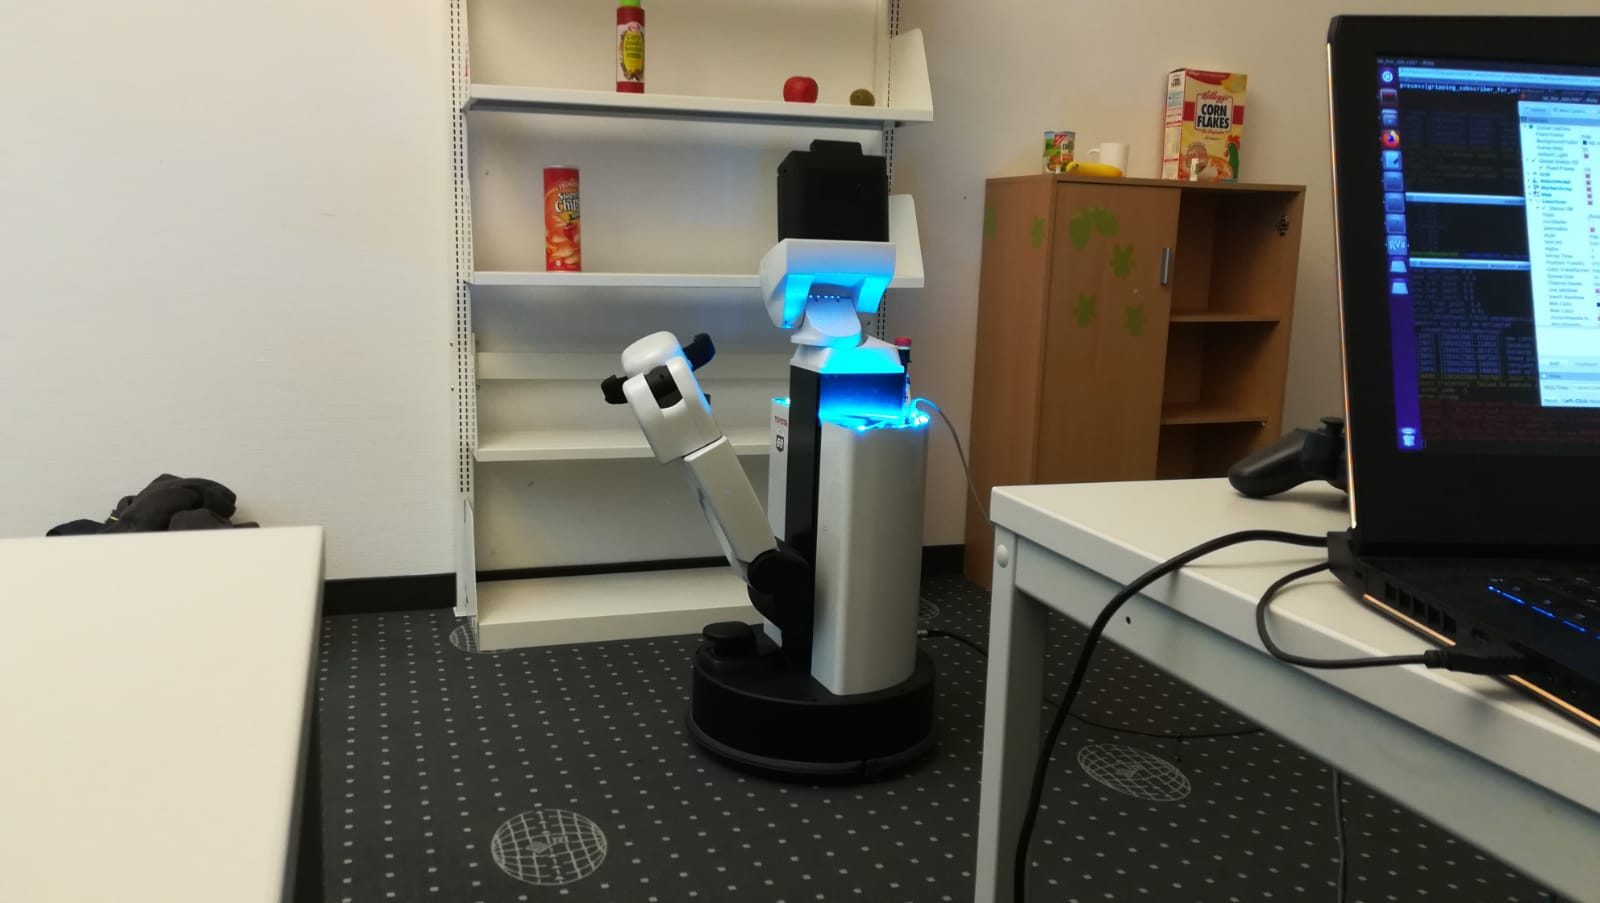
\includegraphics[scale=0.2]{pictures/shelf_scan}
		\caption{HSR scanning the shelf}
	\end{figure}
	
	% Planning confident check
	\begin{planning}
	Planning checks the confident values of detected objects and sorts out objects with too much uncertainty. The data is then transferred to Knowledge.
	\end{planning}
	
	% Knowledge: Store new Objects
	\begin{knowledge}
	Just like after perceiving the table, Knowledge looks into the data of the perceived objects, polishes them, and stores them in the knowledge base.
	\end{knowledge}
	
	\subsection{Place sequence}
	
	% Knowledge: shelf positions
	\begin{knowledge}
	Knowledge again provides Planning with the position of the shelf the robot is standing in front of.
	\end{knowledge}
	
	% navigation: move to shelf
	\begin{navigation}
	The HSR moves to the shelf so it can place the object currently in the gripper.
	\end{navigation}
	
	% Knowledge: Object goal pose
	\begin{knowledge}
	Knowledge now determines the most suitable position for the object which is currently handled. The way this decision is made is explained in the Knowledge function documentation \ref{sec:kn_find_surf}. For now it is enough to know, that Knowledge finds a suitable surface (i.e. shelf floor) as well as a suitable position on that surface for the object.
	\end{knowledge}
	
	% Manipulation: PlaceAction
	\begin{manipulation}
	The procedure for placing an object is very similar to the grasping process. Different modes are available but only the grasp from front mode is actively used. The orientation of the gripper is calculated based on the HSR's rotation and a waypoint is determined to allow smooth in and out movement for shelves. After the object gets released from the gripper its collision is deactivated to avoid problems with the collision box of the gripper during the backward movement. Afterward collision for the object gets enabled again. The actual movement planning and execution are done by \textit{Giskard}.   
	\end{manipulation}
	
	% NLP
	
	% Manipulation: TakePoseAction
	\begin{manipulation}
	After that, the robot is set to the default pose to avoid collisions.
	\end{manipulation}
	% NLP
	
	% Knowledge: table pose
	
	% Knowledge: next_object
	\begin{knowledge}
	Then, Knowledge again finds the nearest object standing on a table that should be handled next.
	\end{knowledge}
	
	% 2x NLP
	\begin{manipulation}
	Grasping the object is once again executed as described under \ref{grasp-object}.
	\end{manipulation}
	
	% Planning: Loop this while some items are left
	\begin{planning}
	Planning then loops this whole procedure from "Grasp Object" on, until either all objects are handled, the HSR can not find any other objects, or the HSR is told via NLP commands to stop its current behavior.
	\end{planning}	
	
	\section{Conclusion}

	The outcome of Storing Groceries can be declared as successful. It has been tested on multiple occasions; like the simulated RoboCup, the demonstrations of the second, and the third milestone. 
	Even though there have been minor setbacks like failing to grasp objects on the first try this leads to showcasing the failure handling capabilities.
	There have also been problems that were caused by hardware issues like the movement of the robot which failed because of the magnet sensors or the problem of \textit{Giskard} avoiding collision with the shelf in the simulation which was seen in the third milestone demo.
	These Problems do not implicate that the plan wasn't working it just had some low-level problems and would have performed the tasks successfully otherwise.
	Since this plan was not stable enough at the time we could still use the real robot, it is hard to say to what extent it would violate the 5 minutes rule. Probably one of the most important next steps would be to look into ways to make the whole process go faster.
	
	\endgroup
	
\end{document}

